

\documentclass{ctexart}
\usepackage{amsmath,bm}
\usepackage{setspace}
\usepackage{xeCJK}
\usepackage{xcolor}
\usepackage{indentfirst}
\usepackage{listings}
\usepackage{graphicx}
\usepackage{subfigure}
\usepackage{amsfonts,amssymb}
\usepackage[a4paper,scale=0.8]{geometry}
\usepackage{hyperref}
\usepackage{float}
\usepackage{listings}
\usepackage{changepage}
\usepackage{longtable}

\usepackage{float}
\definecolor{gray}{rgb}{0.5,0.5,0.5}
\definecolor{dkgreen}{rgb}{.068,.578,.068}
\definecolor{dkpurple}{rgb}{.320,.064,.680}

% set Matlab styles
\lstset{
   language=Matlab,
   numbers=left,
   keywords={break,case,catch,continue,else,elseif,end,for,function,
      global,if,otherwise,persistent,return,switch,try,while},
   basicstyle=\ttfamily,
   keywordstyle=\color{blue}\bfseries,
   commentstyle=\color{dkgreen},
   stringstyle=\color{dkpurple},
   backgroundcolor=\color{white},
   breaklines=true,
   tabsize=4,
   showspaces=false,
   showstringspaces=false,
}
\setCJKmainfont{华光书宋_CNKI}
\newCJKfontfamily\kaiti{华光楷体_CNKI}
\newCJKfontfamily\hei{华光黑体_CNKI}
\newCJKfontfamily\fsong{华光仿宋_CNKI}
\newfontfamily\code{Courier New}
\linespread{1.5} \setlength\parindent{2 em}
\title{\Huge 中国科学技术大学计算机学院\\《数据库系统及应用》实验报告}
\date{\LARGE 2021.07.03}
\begin{document}
\begin{hei}  \maketitle\end{hei}
\begin{figure}[htbp]
    \centering
    
\includegraphics[scale=0.4]{USTC.png}

\end{figure}
\begin{LARGE}\begin{align*}      & \text{实验题目:\underline{数据库应用开发(银行管理系统)}} \\
         & \text{学生姓名:\underline{胡毅翔}}       \\
         & \text{学生学号:\underline{PB18000290}}\end{align*}\end{LARGE}
\par
\par\par
\centerline{\large 计算机实验教学中心制}
\par \centerline {\large 2019年9月}
\newpage
\tableofcontents
\newpage
\section{\hei 概述}
\subsection{\hei 系统目标}
本次实验目标为实现一个银行业务管理系统。系统需要实现以下功能:
\begin{enumerate}
    \item 正确连接数据库与客户端。
    \item 客户端为用户(银行管理人员)提供银行业务的图形操作界面,具体业务包括:
    \begin{enumerate}
        \item 客户管理;
        \item 账户管理;
        \item 贷款管理;
        \item 业务统计。
    \end{enumerate}
    本次实现的客户端还实现了支行管理,员工管理的功能。
    \item 业务信息实时反应到数据库上。
    \item 保证客户端可以避免或处理一些可预知的错误,并给予用户提示。
\end{enumerate}
\subsection{\hei 需求说明}
\subsubsection{\hei 数据需求}
银行有多个支行。各个支行位于某个城市,每个支行有唯一的名字。银行要监控每个支
行的资产。 银行的客户通过其身份证号来标识。银行存储每个客户的姓名、联系电话以及
家庭住址。为了安全起见,银行还要求客户提供一位联系人的信息,包括联系人姓名、手机
号、Email 以及与客户的关系。客户可以有帐户,并且可以贷款。客户可能和某个银行员工
发生联系,该员工是此客户的贷款负责人或银行帐户负责人。 银行员工也通过身份证号来
标识。员工分为部门经理和普通员工,每个部门经理都负责领导其所在部门的员工,并且每
个员工只允许在一个部门内工作。每个支行的管理机构存储每个员工的姓名、电话号码、家
庭地址、所在的部门号、部门名称、部门类型及部门经理的身份证号。银行还需知道每个员
工开始工作的日期,由此日期可以推知员工的雇佣期。 银行提供两类帐户——储蓄帐户和
支票帐户。帐户可以由多个客户所共有,一个客户也可开设多个账户,但在一个支行内最多
只能开设一个储蓄账户和一个支票账户。每个帐户被赋以唯一的帐户号。银行记录每个帐户
的余额、开户日期、开户的支行名以及每个帐户所有者访问该帐户的最近日期。另外,每个
储蓄帐户有利率和货币类型,且每个支票帐户有透支额。 每笔贷款由某个分支机构发放,
能被一个或多个客户所共有。每笔贷款用唯一的贷款号标识。银行需要知道每笔贷款所贷金
额以及逐次支付的情况(银行将贷款分几次付给客户)。虽然贷款号不能唯一标识银行所有
为贷款所付的款项,但可以唯一标识为某贷款所付的款项。对每次的付款需要记录日期和金
额。
\subsubsection{\hei 功能需求}
\begin{enumerate}
    \item 客户管理:提供客户所有信息的增、删、改、查功能;如果客户存在着关联账户或者贷款记录则不允许删除;
    \item 账户管理:提供账户开户、销户、修改、查询功能,包括储蓄账户和支票账户;账户号不允许修改;
    \item 贷款管理:提供贷款信息的增、删、查功能,提供贷款发放功能;贷款信息一旦添加成
    功后不允许修改;要求能查询每笔贷款的当前状态(未开始发放、发放中、已全部发
    放);处于发放中状态的贷款记录不允许删除;
    \item 业务统计:按业务分类(储蓄、贷款)和时间(月、季、年)统计各个支行的业务总金
    额和用户数,统计的结果以表格形式展示。
\end{enumerate}
\subsection{\hei 本报告的主要贡献}
\begin{enumerate}
    \item 介绍本系统的设计目标及功能需求;
    \item 介绍本系统的总体设计思路,系统工作流程,数据库设计;
    \item 介绍本系统各个功能模块的设计实现;
    \item 演示本系统运行结果;
    \item 总结系统设计过程中的问题及解决方案;
    \item 总结本系统开发过程中的体会及感悟。
\end{enumerate}
\section{\hei 实验环境}
\begin{enumerate}
    \item PC一台
    \item Windows 10操作系统
    \item Eclipse IDE for Java Developers 2020-03 (4.15.0)
    \item Visual Studio Code 1.56.2
    \item Oracle 11g Release 2 (11.2) for Microsoft Windows x64 (64-Bit)
    \item Java 16.0.1 2021-04-20
    \item PL/SQL Developer 64 bit 13.0.2.1898
\end{enumerate}
\section{\hei 总体设计}
\subsection{\hei 系统模块结构}
本系统采用的数据库应用系统结构是以前端为主的两层式结构。后端服务器只提供数据服务(数据存储及维护)。
商业服务(数据处理与检查)及操作界面服务(数据的输入与显示)由前端客户端来完成。具体模块结构图如下:
\begin{figure}[H]
    \centering
    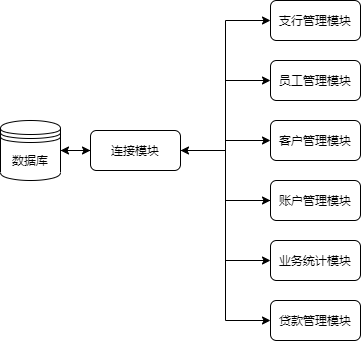
\includegraphics[scale=0.7]{Untitled D123iagram.png}
    \caption{ER图}
\end{figure}
\par 前端分为连接模块,支行管理模块,员工管理模块,客户管理模块,账户管理模块,贷款管理模块,
业务统计模块。
\par 连接模块控制客户端与数据库的连接,登录后建立子模块与数据库的连接,登出后断开子模块与数据库的连接,退出后关闭银行业务管理系统。
\par 支行管理模块在登录成功后,提供支行的增删改查功能。
\par 员工管理模块在登录成功后,提供员工信息的增删改查功能,并自动检查是否有员工所在部门及支行信息。
\par 客户管理模块在登录成功后,提供客户信息的增删改查功能,并检查客户负责人是否存在。
\par 账户管理模块在登录成功后,提供账户信息的增删改查功能,并检查账户所有人及所在银行是否存在。
\par 贷款管理模块在登录成功后,提供贷款信息的增删改查功能,此外还包括逐次发放贷款功能,记录贷款发放状态(未发放,发放中,已全部发放),保证在发放中的贷款记录不能删除。
\par 业务统计模块在登录成功后,提供各个支行贷款,储蓄逐月,逐季,逐年的业务金额及客户数统计,提供表格形式及折线图形式的统计结果。
\subsection{\hei 系统工作流程}
系统工作流程图,如下:
\begin{figure}[H]
    \centering
    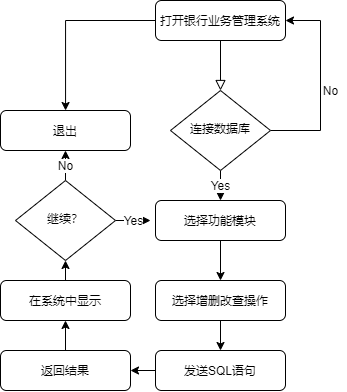
\includegraphics[scale=0.7]{Untitled Diagram (1).png}
    \caption{系统工作流程图}
\end{figure}
\begin{enumerate}
    \item 打开银行业务管理系统;
    \item 通过登录,连接数据库;
    \item 选择需要操作的功能模块;
    \item 设置查询条件,点击查询,客户端向数据库发出$SQL$查询语句,数据库返回查询结果,得到该模块的满足条件的所有实例(若条件为空,则返回所有实例),客户端以表格形式显示;
    \item 点击添加,输入信息,客户端向数据库发出$SQL$插入语句,数据库尝试插入,增加新的实例,若添加失败,返回错误信息并显示给用户;
    \item 勾选实例并点击删除,客户端向数据库发出$SQL$删除语句,若实例可删除,则在数据库中删除,否则返回错误信息并显示给用户;
    \item 勾选实例并点击修改,客户端向数据库发出$SQL$修改语句,若实例可修改,则在数据库中修改,否则返回错误信息并显示给用户;
    \item 勾选统计条件,生成业务统计查询表,点击业务金额曲线或客户数曲线生成对应曲线;
    \item 通过登出,断开与数据库的连接;
    \item 通过退出,退出本系统。
\end{enumerate}
\subsection{\hei 数据库设计}
数据库设计的ER图,如下:
\begin{figure}[H]
    \centering
    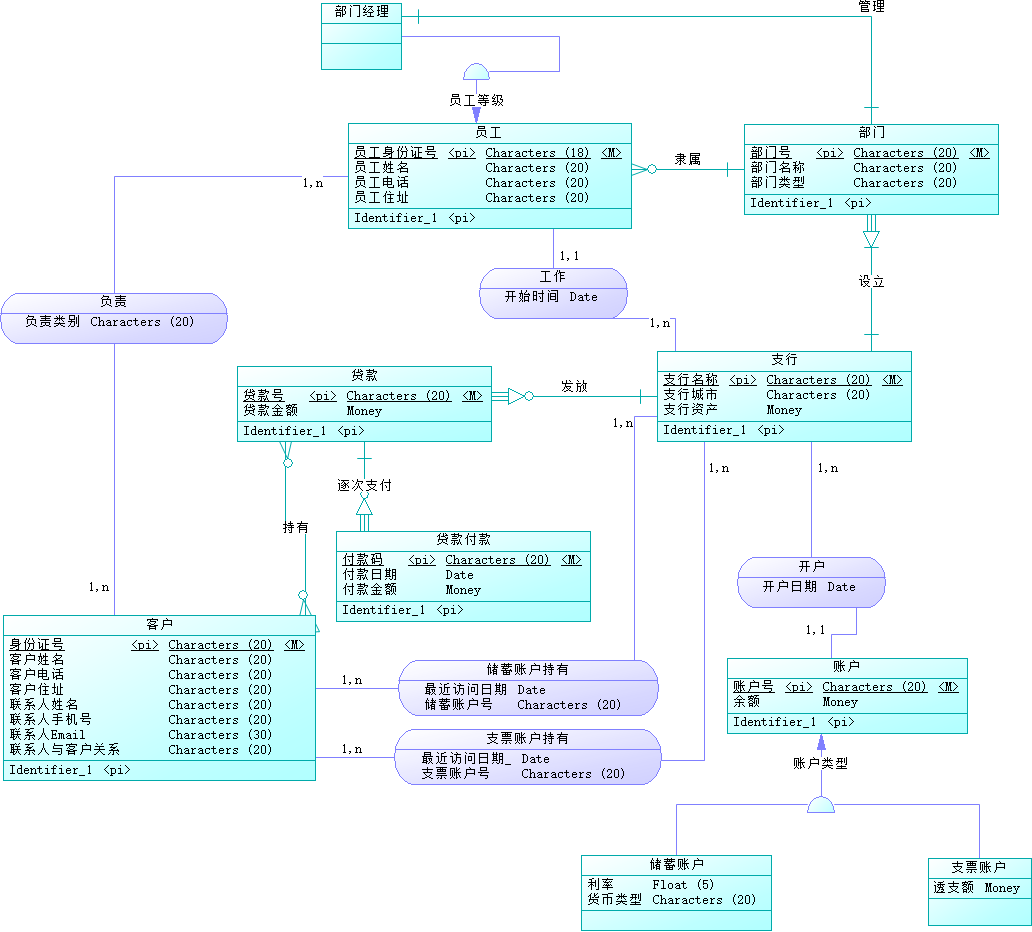
\includegraphics[scale=0.7]{er.png}
    \caption{ER图}
\end{figure}
逻辑数据库结构,如下:
\begin{figure}[H]
    \centering
    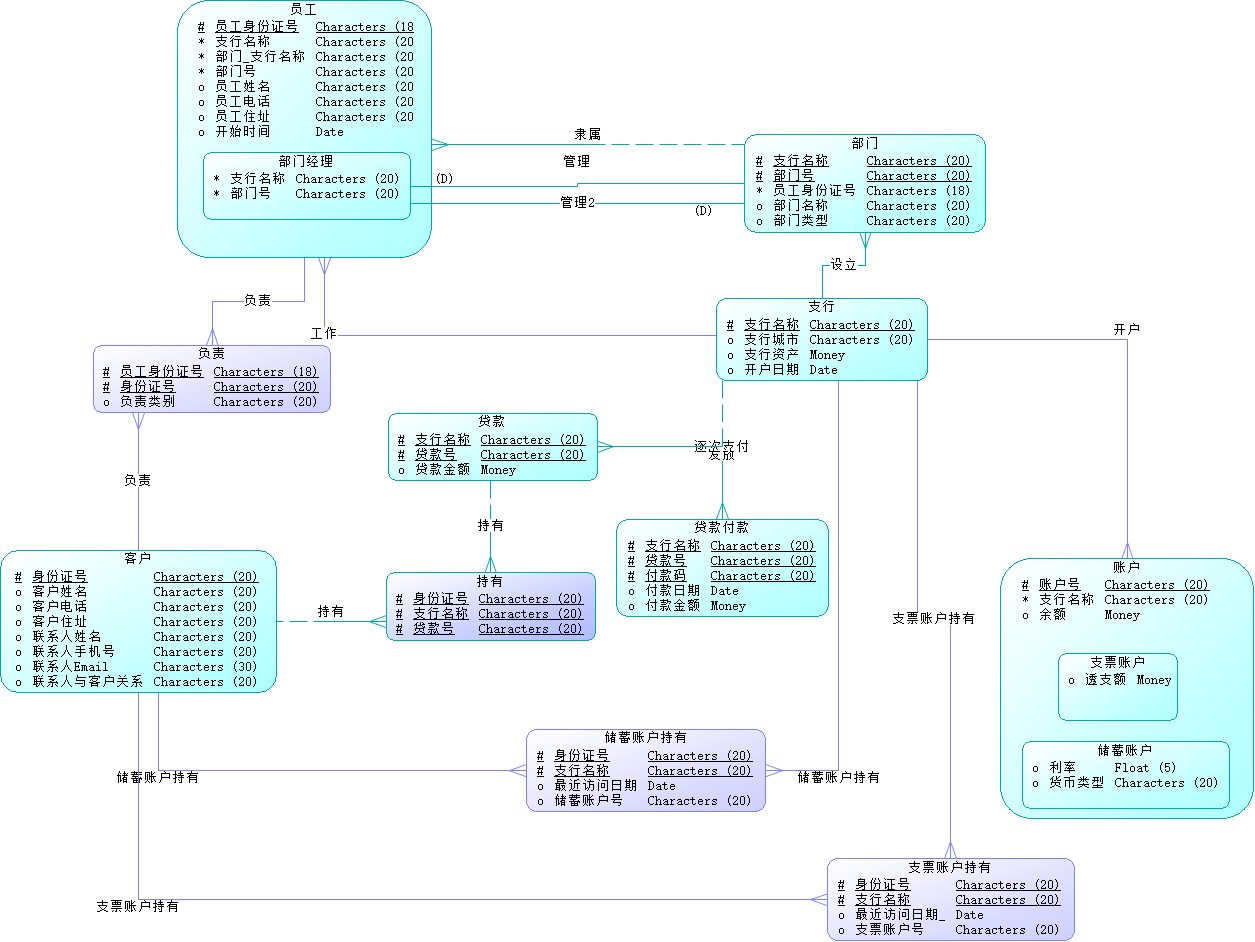
\includegraphics[scale=0.6]{logi.png}
    \caption{逻辑数据库结构}
\end{figure}
最终的物理数据库结构,如下:
\begin{figure}[H]
    \centering
    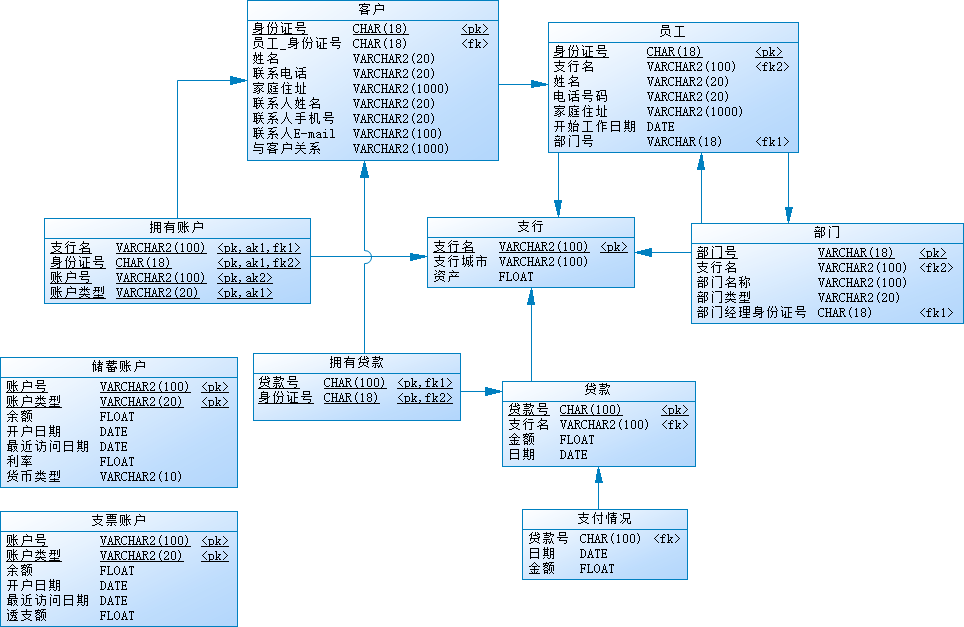
\includegraphics[scale=0.6]{phy.png}
    \caption{物理数据库结构}
\end{figure}
在物理数据库结构中,对储蓄账户和支票账户的管理更为简洁,通过将表储蓄账户(或支票账户)中的账户号和账户类型的修改与拥有账户表
中的这两项的修改设为原子操作,避免了过多表带来的额外存储代价和更新代价。
\section{\hei 详细设计}
\subsection{\hei 连接模块}
该模块用于控制客户端与数据库的连接,具体工作流程如下:
\begin{enumerate}
    \item 点击“菜单”;
    \item 选择“登陆”;
    \item 在弹出的新对话框中输入“端口”(Port),“数据库名称”(SID),“用户名”(User Name),“密码”(Password),点击“确定”;
    \item 客户端根据用户提供的连接信息尝试连接数据库,若成功,则用户可以继续调用子模块,进行银行业务管理;若失败,则返回错误信息;
    \item 点击“菜单”$\rightarrow$“登出”,断开客户端与数据库的连接;
    \item 点击“菜单”$\rightarrow$“退出”,退出本系统。
\end{enumerate}
\subsection{\hei 支行管理模块}
该模块提供支行信息的增删改查功能,具体工作流程如下:
\begin{enumerate}
    \item 点击子菜单栏中的“支行管理”,进入支行信息管理界面;
    \item 点击“添加”,在弹出的对话框中输入“支行名”,“支行城市”,“资产”,点击“确定”,添加新的支行;
    \item 点击“查询”,返回当前所有支行信息(以表格形式呈现),若在点击“查询”前,设置查询条件,则返回满足条件的支行信息;
    \item 点击查询结果最左侧的方框,勾选想要删除的支行信息(可多选),点击“删除”。若该支行不存在员工等信息的约束,且满足删除条件,则在数据库中删除该支行,否则返回错误信息;
    \item 点击查询结果表,双击任意表项,可以直接对数据进行修改,修改后,勾选想要修改的支行信息(可多选),点击“修改”。若满足修改条件,则在数据库中修改该支行的信息,否则返回错误信息。
\end{enumerate}
\subsection{\hei 员工管理模块}
该模块提供员工信息的增删改查功能,具体工作流程如下:
\begin{enumerate}
    \item 点击子菜单栏中的“员工管理”,进入员工信息管理界面;
    \item 点击“添加”,在弹出的对话框中输入“身份证号”,“支行名”,“姓名”,“电话号码”,“家庭住址”,“开始工作时间”,“部门号”,点击“确定”,若满足添加条件(有该支行和部门,且身份证号唯一),添加新的员工;
    \item 点击“查询”,返回当前所有员工信息(以表格形式呈现),若在点击“查询”前,设置查询条件,则返回满足条件的员工信息;
    \item 点击查询结果最左侧的方框,勾选想要删除的员工信息(可多选),点击“删除”。若该员工不存在客户等信息的约束,且满足删除条件,则在数据库中删除该员工,否则返回错误信息;
    \item 点击查询结果表,双击任意表项,可以直接对数据进行修改,修改后,勾选想要修改的员工信息(可多选),点击“修改”。若满足修改条件,则在数据库中修改该员工的信息,否则返回错误信息。
\end{enumerate}
\subsection{\hei 客户管理模块}
该模块提供客户信息的增删改查功能,具体工作流程如下:
\begin{enumerate}
    \item 点击子菜单栏中的“客户管理”,进入客户信息管理界面;
    \item 点击“添加”,在弹出的对话框中输入“身份证号”,“负责员工身份证号”,“姓名”,“联系电话”,“家庭住址”,“联系人姓名”,“联系人手机号”,“联系人E-mail”,“与客户关系”点击“确定”,若满足添加条件(有该员工,且身份证号唯一),添加新的客户;
    \item 点击“查询”,返回当前所有客户信息(以表格形式呈现),若在点击“查询”前,设置查询条件,则返回满足条件的客户信息;
    \item 点击查询结果最左侧的方框,勾选想要删除的客户信息(可多选),点击“删除”。若该客户不存在贷款等信息的约束,且满足删除条件,则在数据库中删除该客户,否则返回错误信息;
    \item 点击查询结果表,双击任意表项,可以直接对数据进行修改,修改后,勾选想要修改的客户信息(可多选),点击“修改”。若满足修改条件,则在数据库中修改该客户的信息,否则返回错误信息。
\end{enumerate}
\subsection{\hei 账户管理模块}
该模块提供账户信息的增删改查功能,具体工作流程分储蓄账户和支票账户两部分。
\subsubsection{\hei 储蓄账户}
\begin{enumerate}
    \item 点击子菜单栏中的“账户管理”,进入账户信息管理界面;
    \item 下拉选择“储蓄账户”;
    \item 点击“开户”,在弹出的对话框中输入“账户号”,“余额”,“开户日期”,“最近访问日期”,“利率”,“货币类型”,“支行名”,“身份证号”
    ,点击“确定”,若满足添加条件(账户号唯一,且该用户在该支行未拥有储蓄账户),添加新的储蓄账户;
    \item 点击“查询”,返回当前所有储蓄账户信息(以表格形式呈现),若在点击“查询”前,设置查询条件,则返回满足条件的储蓄账户信息;
    \item 点击查询结果最左侧的方框,勾选想要删除的储蓄账户信息(可多选),点击“删除”。若该储蓄账户满足删除条件,则在数据库中删除该储蓄账户,否则返回错误信息;
    \item 点击查询结果表,双击任意表项,可以直接对数据进行修改,修改后,勾选想要修改的储蓄账户信息(可多选),点击“修改”。若满足修改条件,则在数据库中修改该储蓄账户的信息,否则返回错误信息。
\end{enumerate}
\subsubsection{\hei 支票账户}
\begin{enumerate}
    \item 点击子菜单栏中的“账户管理”,进入账户信息管理界面;
    \item 下拉选择“支票账户”;
    \item 点击“开户”,在弹出的对话框中输入“账户号”,“余额”,“开户日期”,“最近访问日期”,“透支额”,“支行名”,“身份证号”
    ,点击“确定”,若满足添加条件(账户号唯一,且该用户在该支行未拥有支票账户),添加新的支票账户;
    \item 点击“查询”,返回当前所有支票账户信息(以表格形式呈现),若在点击“查询”前,设置查询条件,则返回满足条件的支票账户信息;
    \item 点击查询结果最左侧的方框,勾选想要删除的支票账户信息(可多选),点击“删除”。若该支票账户满足删除条件,则在数据库中删除该支票账户,否则返回错误信息;
    \item 点击查询结果表,双击任意表项,可以直接对数据进行修改,修改后,勾选想要修改的支票账户信息(可多选),点击“修改”。若满足修改条件,则在数据库中修改该支票账户的信息,否则返回错误信息。
\end{enumerate}
\subsection{\hei 贷款管理模块}
该模块提供贷款业务信息的增删查功能,具体工作流程如下:
\begin{enumerate}
    \item 点击子菜单栏中的“贷款管理”,进入账户贷款业务管理界面;
    \item 点击“添加”,在弹出的对话框中输入“贷款号”,“支行名”,“金额”,“日期”,“身份证号”,点击“确定”,若满足添加条件(有该支行和身份证号,且贷款号唯一),添加新的贷款;
    \item 点击“查询”,返回当前所有贷款信息(包括贷款发放状态:未开始发放,发放中,已全部发放)(以表格形式呈现),若在点击“查询”前,设置查询条件,则返回满足条件的贷款业务信息;
    \item 点击查询结果最左侧的方框,勾选想要删除的贷款业务信息(可多选),点击“删除”。若该贷款业务满足删除条件(发放状态不是发放中且,对应的支票账户中余额充足),则在数据库中删除该贷款业务,
    并对该业务对应的支票账户进行修改,否则返回错误信息;
    \item 点击查询结果最左侧的方框,勾选想要发放贷款的贷款业务,点击“发放”,在弹出的对话框中输入“日期”,“金额”,点击“确定”,若该贷款业务满足发放条件(未全部发放),发放贷款,并修改相应贷款发放状态,及对应支票账户,
    否则返回错误信息。
\end{enumerate}
\subsection{\hei 业务统计模块}
该模块提供业务统计功能,具体工作流程如下:
\begin{enumerate}
    \item 点击子菜单栏中的“业务统计”,进入业务统计界面;
    \item 下拉“账户类型”,选择“储蓄账户”或“贷款”;
    \item 下拉“时间跨度”,选择“月”,“季”,“年”;
    \item 下拉“支行”,选择进行统计的支行名;
    \item 点击“查询”,根据设置的查询条件,进行业务统计,返回对应范围的业务金额数据及用户数数据,以表格形式显示;
    \item 点击“业务金额曲线”或“客户数曲线”,生成统计结果的折线图。
\end{enumerate}
\section{\hei 实现与测试}
该部分包括本次实验实现的银行业务管理系统的演示结果,以及对一些已知情况的处理的测试。
\subsection{\hei 实现结果}
\subsubsection{\hei 连接模块}
选择“菜单”$\rightarrow$“登陆”;
\par 
\begin{figure}[H]
    \centering
    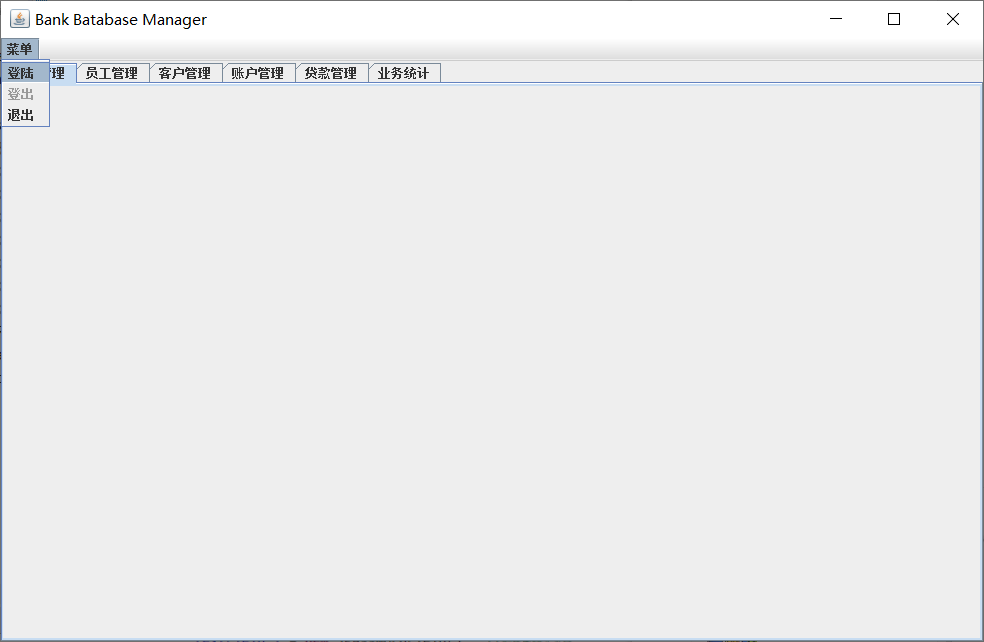
\includegraphics[scale=0.2]{deng.png}
    \caption{登录}
\end{figure}
输入连接的数据库,端口,账号及密码;
\par 
\begin{figure}[H]
    \centering
    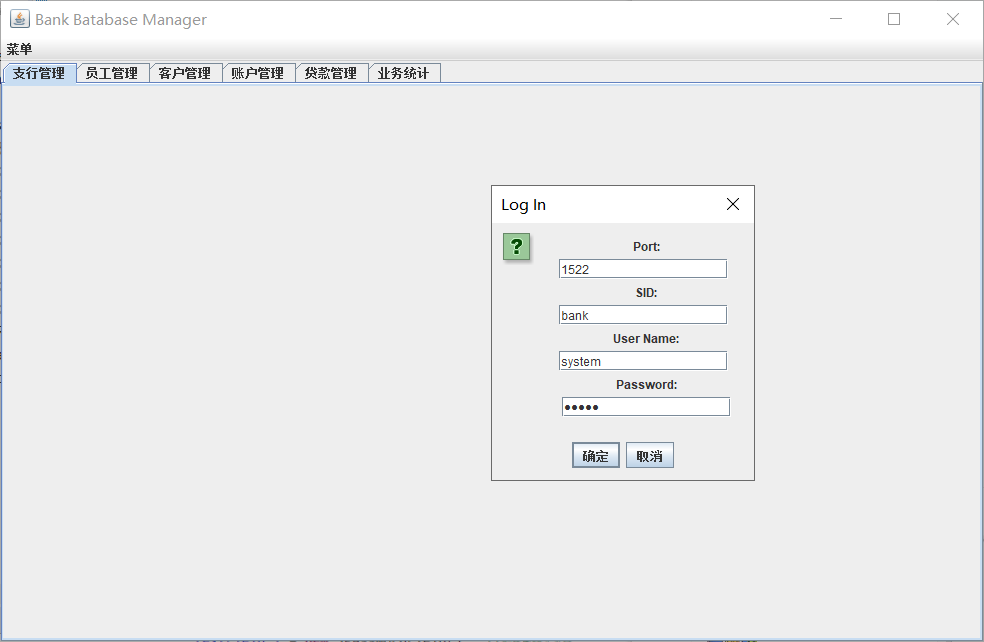
\includegraphics[scale=0.2]{lu.png}
    \caption{连接数据库}
\end{figure}
完成登录。
\par “登出”及“退出”同理。
\subsubsection{\hei 支行管理模块}
在子菜单栏选择“支行管理模块”;
\par 
\begin{figure}[H]
    \centering
    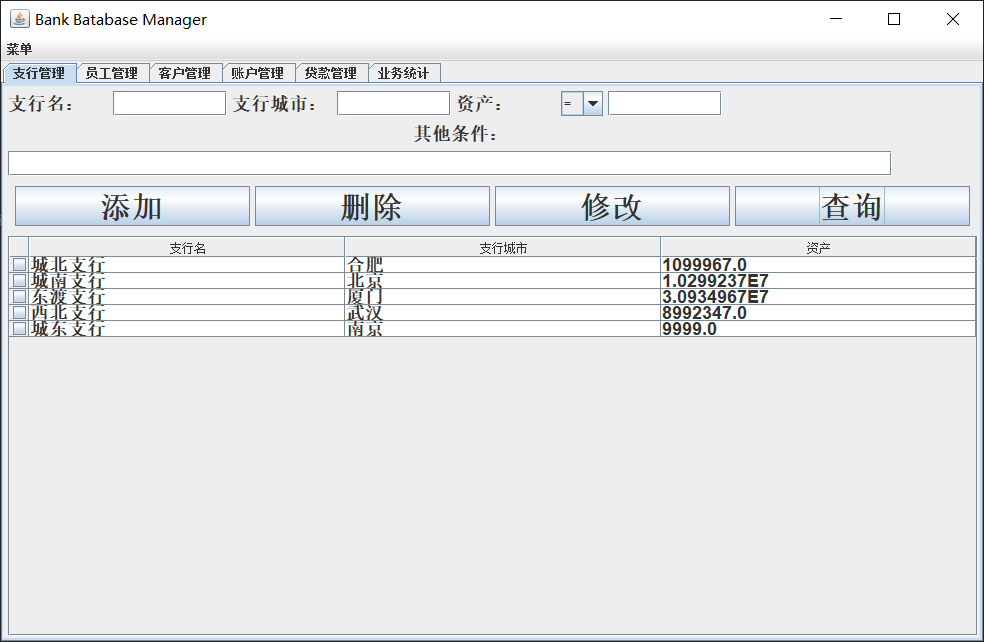
\includegraphics[scale=0.2]{zhgl1.png}
    \caption{支行管理模块}
\end{figure}
双击表项,进入编辑模式,进行修改,完成后勾选并点击“修改”;
\begin{figure}[H]
    \centering
    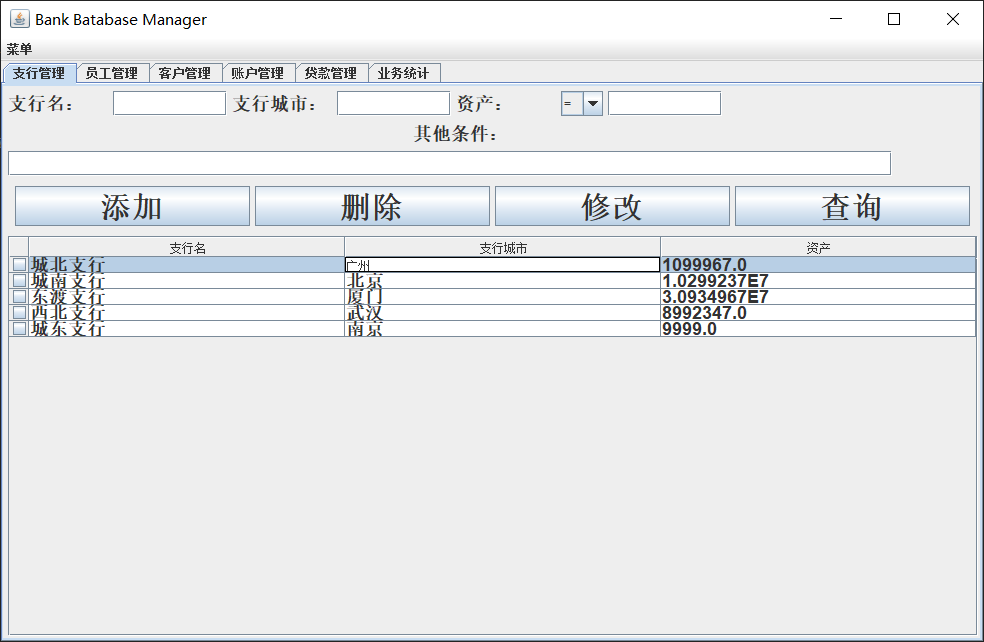
\includegraphics[scale=0.2]{zhgl2.png}
    \caption{支行管理模块-修改演示}
\end{figure}
\par 
设置查询条件(此处设置支行资产<2000000),点击“查询”;
\begin{figure}[H]
    \centering
    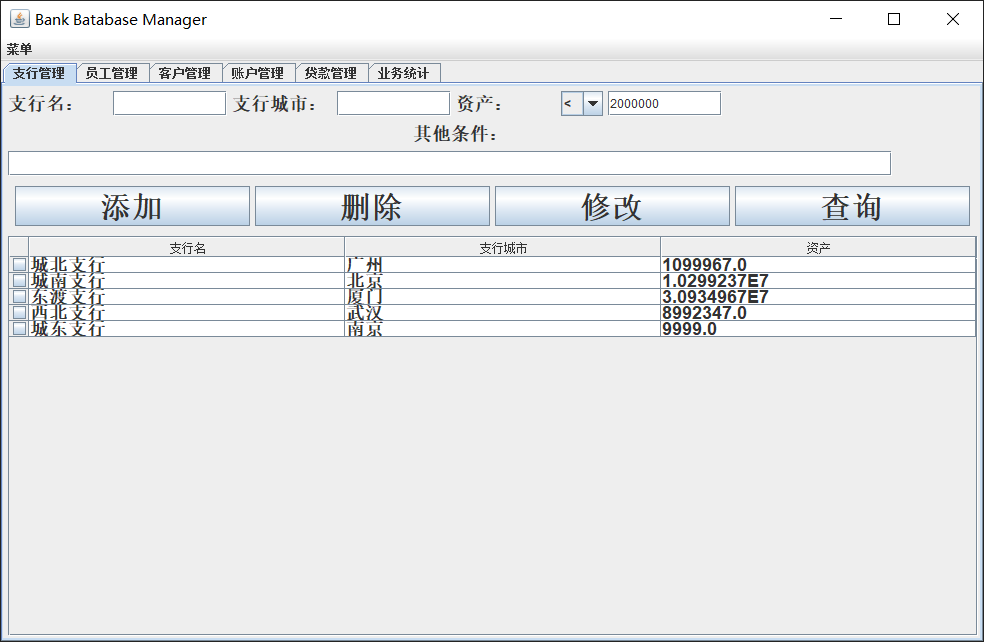
\includegraphics[scale=0.2]{zhgl3.png}
    \caption{支行管理模块-查询演示1}
\end{figure}
\par 
结果为:
\begin{figure}[H]
    \centering
    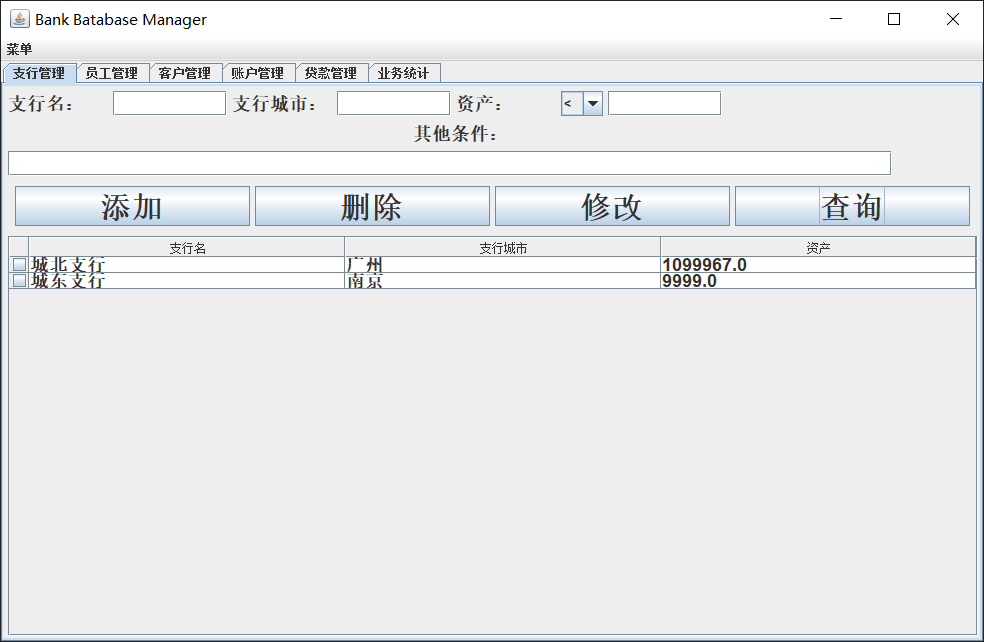
\includegraphics[scale=0.2]{zhgl.png}
    \caption{支行管理模块-查询演示2}
\end{figure}
\par 
勾选“城东支行”,点击“删除”;
\begin{figure}[H]
    \centering
    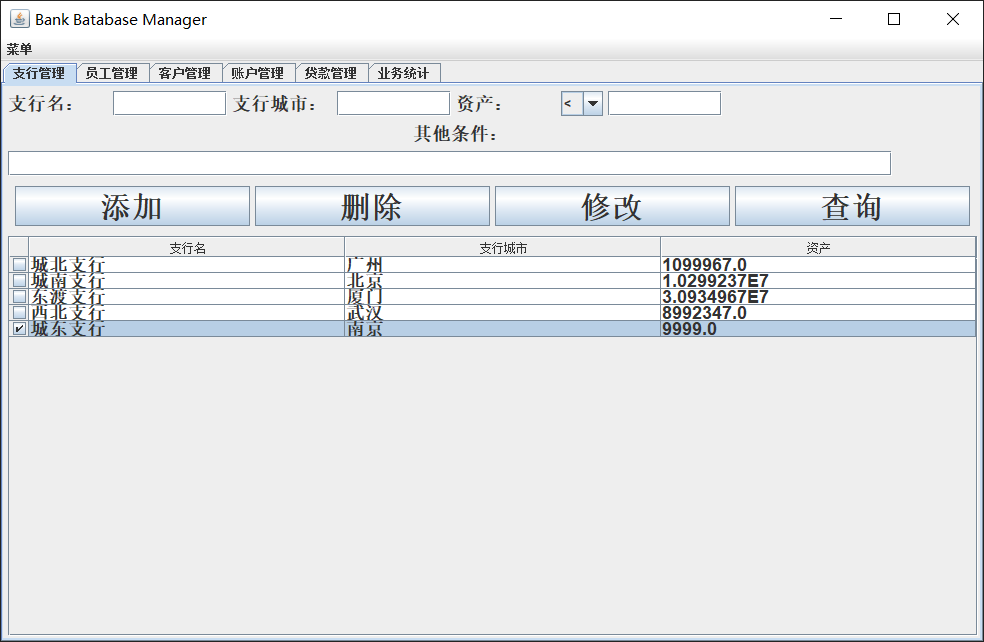
\includegraphics[scale=0.2]{zhgl4.png}
    \caption{支行管理模块-删除演示1}
\end{figure}
\par 
结果为:
\begin{figure}[H]
    \centering
    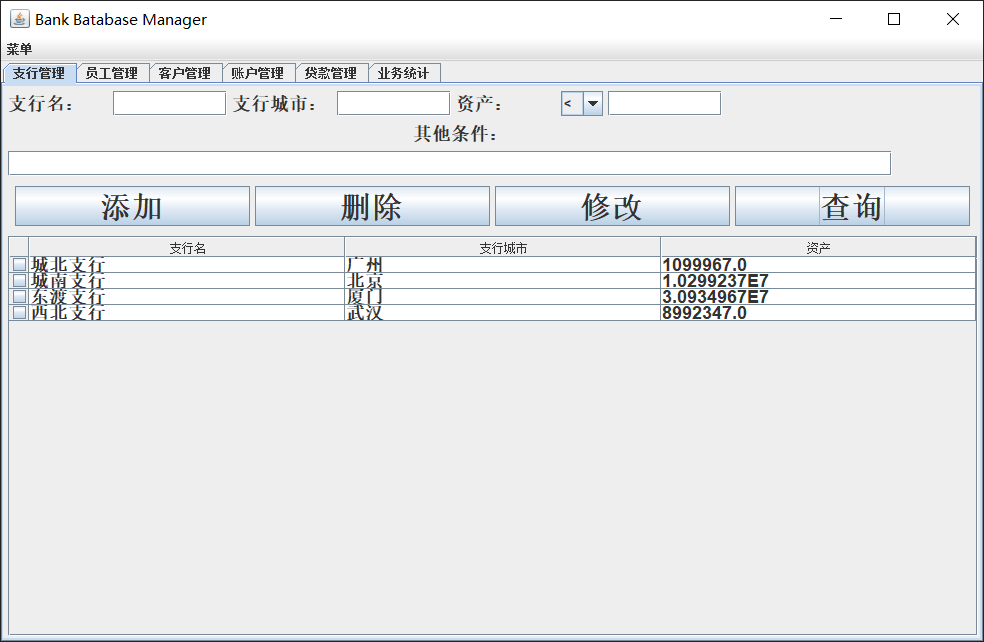
\includegraphics[scale=0.2]{zhgl5.png}
    \caption{支行管理模块-删除演示2}
\end{figure}
\par 
点击“添加”,输入相应信息,点击“确定”;
\begin{figure}[H]
    \centering
    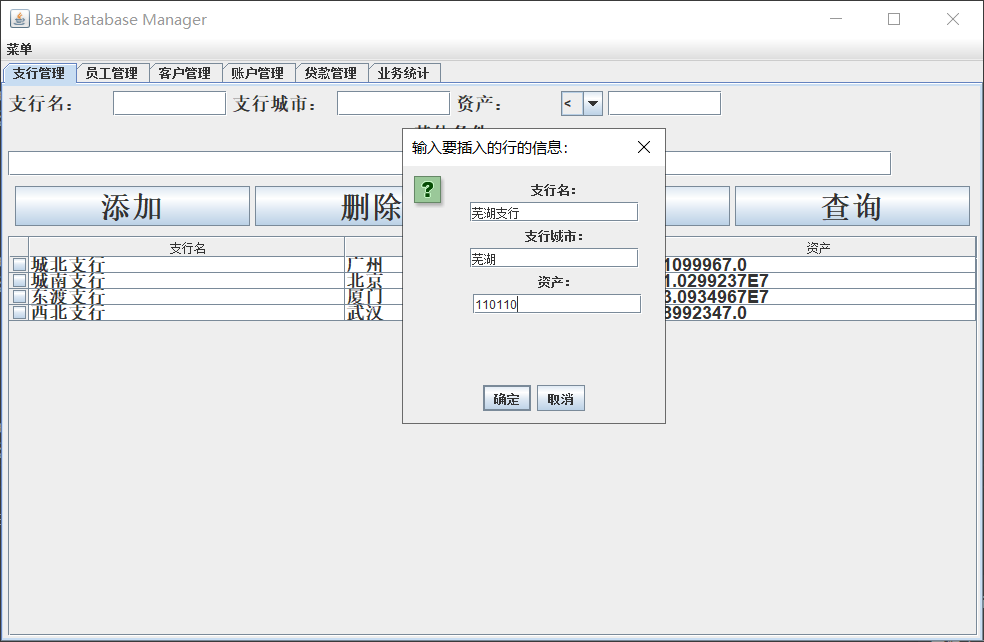
\includegraphics[scale=0.2]{zhgl6.png}
    \caption{支行管理模块-添加演示1}
\end{figure}
\par 
结果为:
\begin{figure}[H]
    \centering
    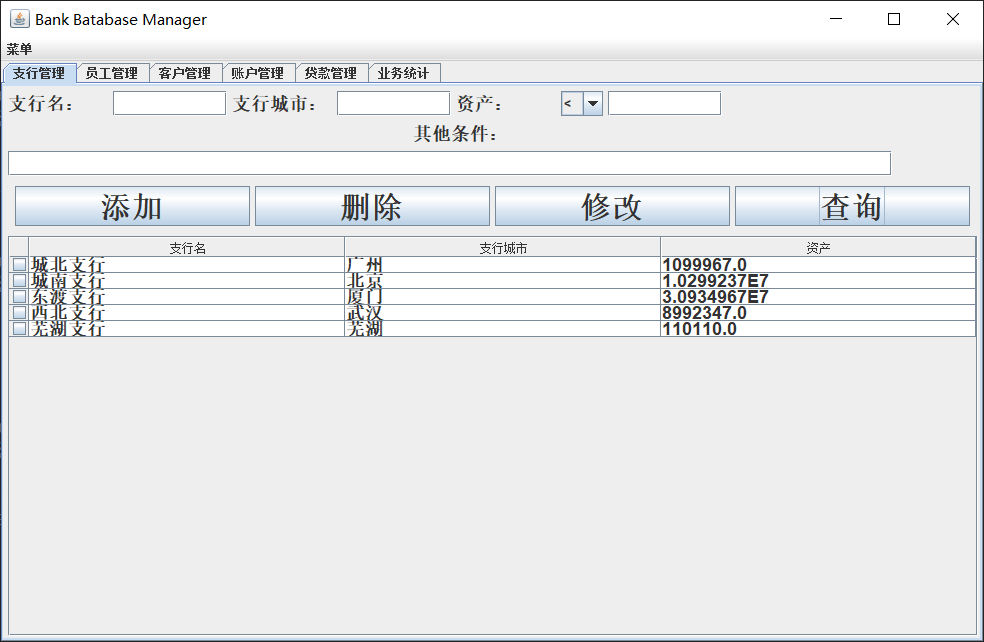
\includegraphics[scale=0.2]{zhgl7.png}
    \caption{支行管理模块-添加演示2}
\end{figure}
\subsubsection{\hei 员工管理模块}
在子菜单栏选择“员工管理模块”;
\par 
\begin{figure}[H]
    \centering
    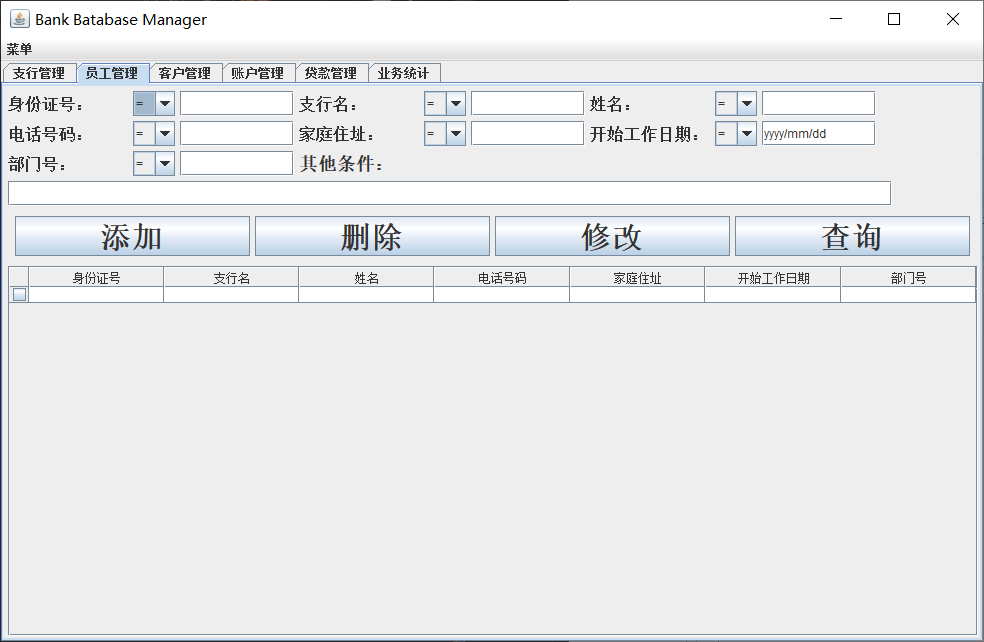
\includegraphics[scale=0.2]{yggl.png}
    \caption{员工管理模块}
\end{figure}
增删改查功能与支行管理模块类似。
\subsubsection{\hei 客户管理模块}
在子菜单栏选择“客户管理模块”;
\par 
\begin{figure}[H]
    \centering
    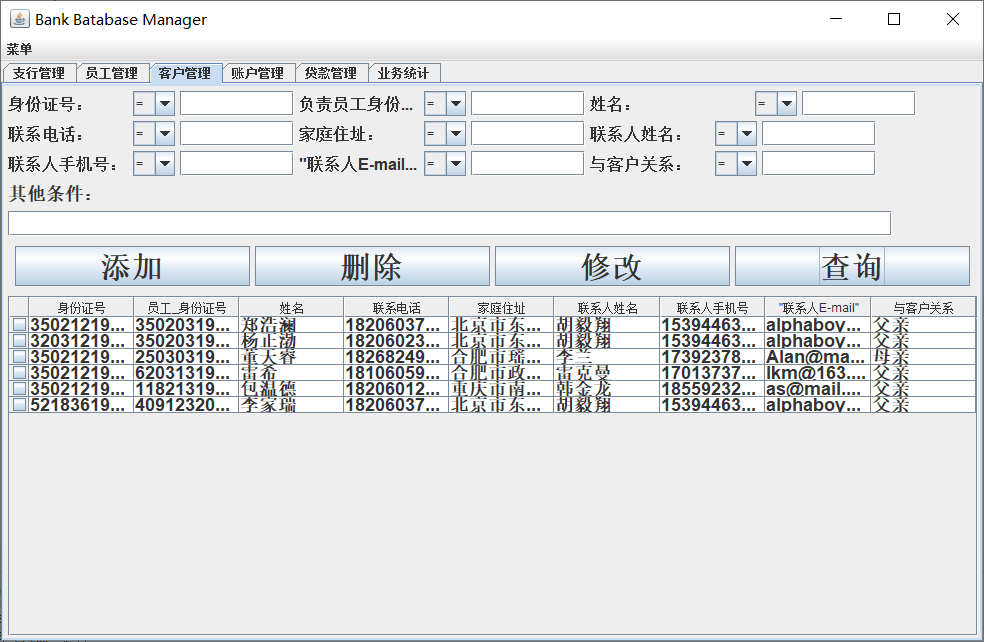
\includegraphics[scale=0.2]{khgl.png}
    \caption{客户管理模块}
\end{figure}
增删改查功能与支行管理模块类似。
\subsubsection{\hei 账户管理模块}
在子菜单栏选择“账户管理模块”;
\par 
\begin{figure}[H]
    \centering
    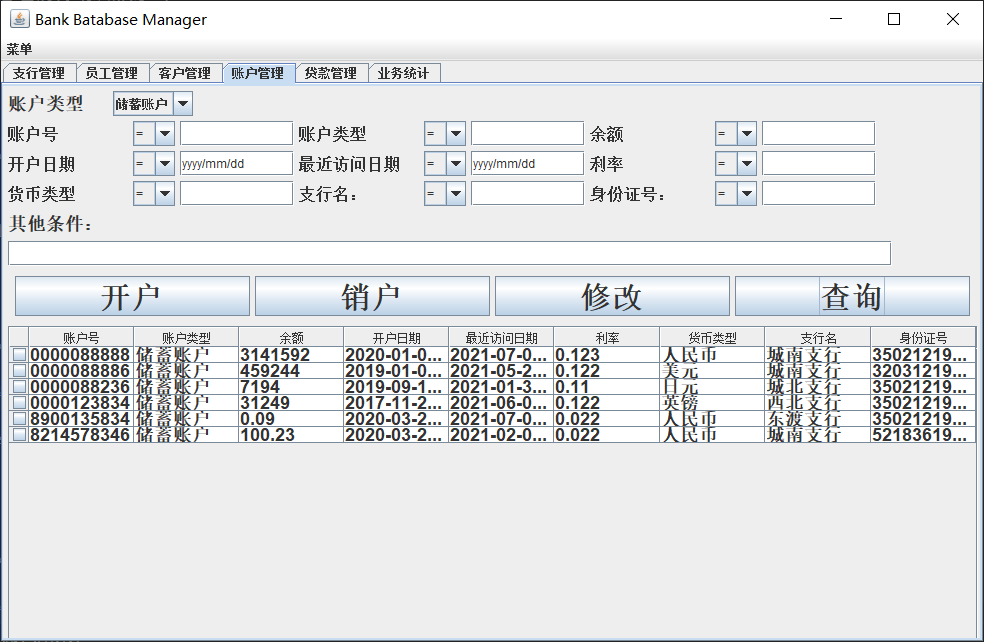
\includegraphics[scale=0.2]{zhanghu.png}
    \caption{账户管理模块}
\end{figure}
增删改查功能与支行管理模块类似。
\subsubsection{\hei 贷款管理模块}
在子菜单栏选择“贷款管理模块”;
\par 
\begin{figure}[H]
    \centering
    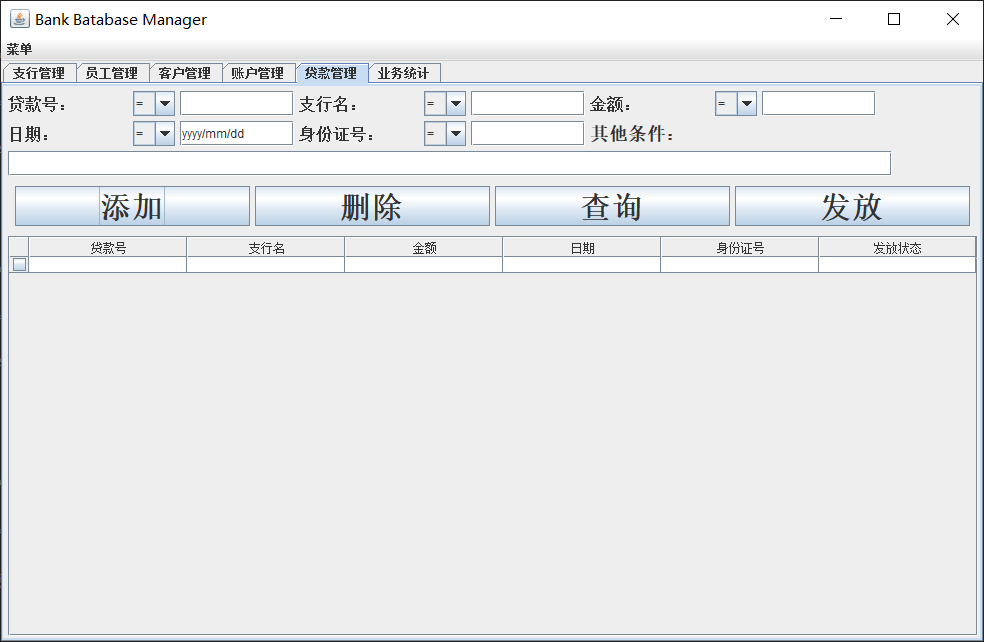
\includegraphics[scale=0.2]{dk.png}
    \caption{贷款管理模块}
\end{figure}
点击“添加”,增加贷款业务;
\begin{figure}[H]
    \centering
    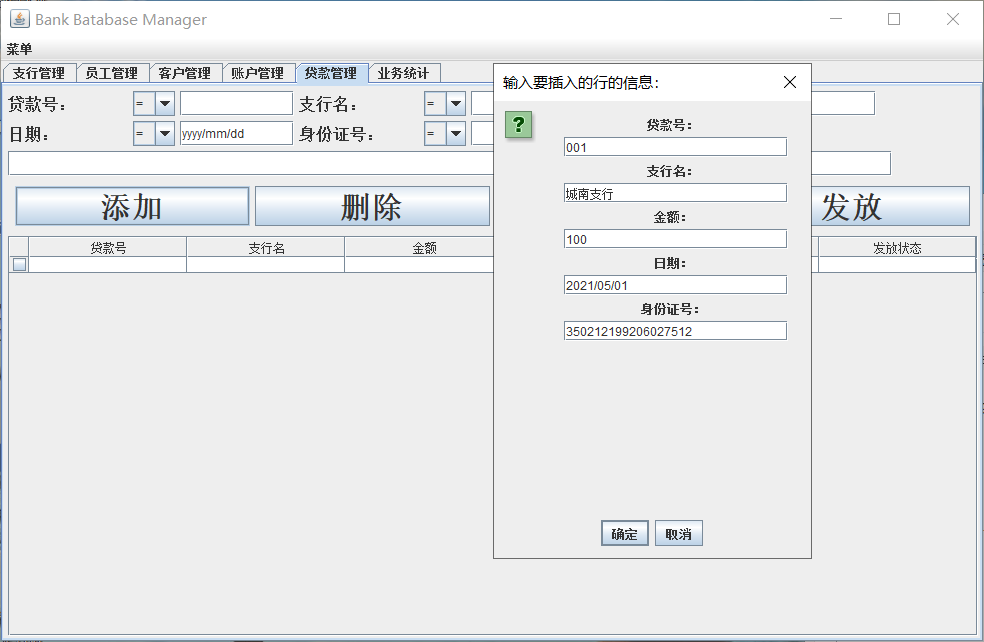
\includegraphics[scale=0.2]{dk1.png}
    \caption{贷款管理模块-添加}
\end{figure}
\par
点击“发放”,发放贷款;
\begin{figure}[H]
    \centering
    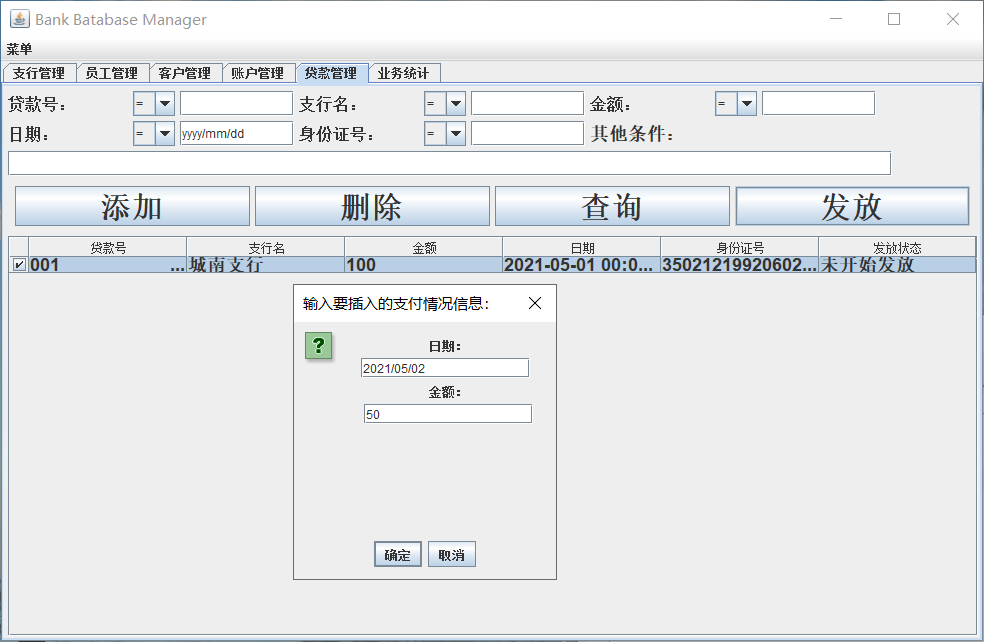
\includegraphics[scale=0.2]{dk2.png}
    \caption{账户管理模块-发放}
\end{figure}
\par
其余功能与支行管理模块类似。
\subsubsection{\hei 业务统计模块}
在子菜单栏选择“贷款管理模块”;
\par 
\begin{figure}[H]
    \centering
    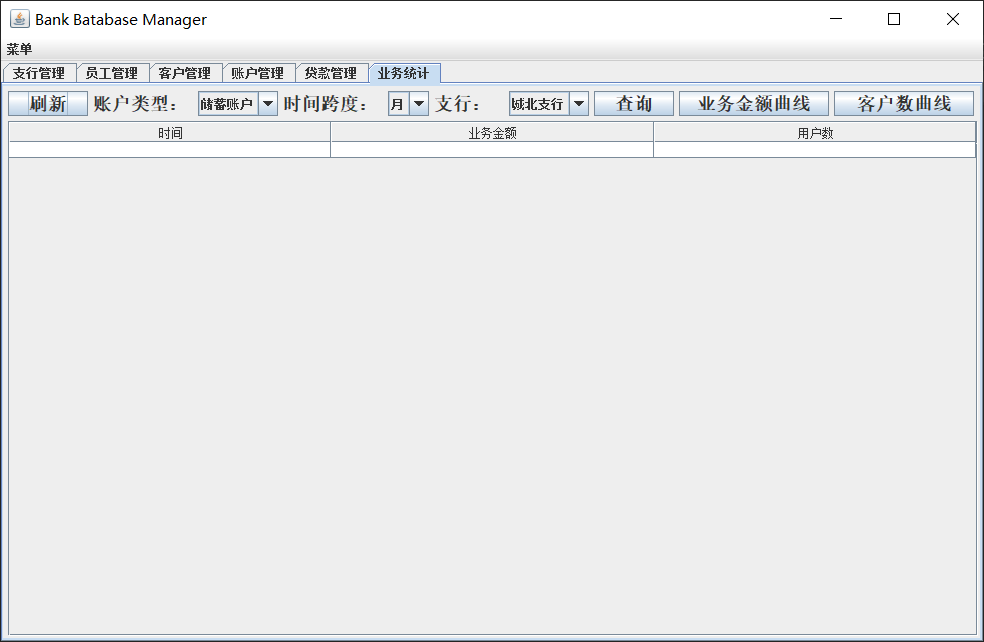
\includegraphics[scale=0.2]{tj.png}
    \caption{业务统计模块}
\end{figure}
选择“储蓄账户”,“年”,“城南支行”,点击“查询”,结果如下:
\par 
\begin{figure}[H]
    \centering
    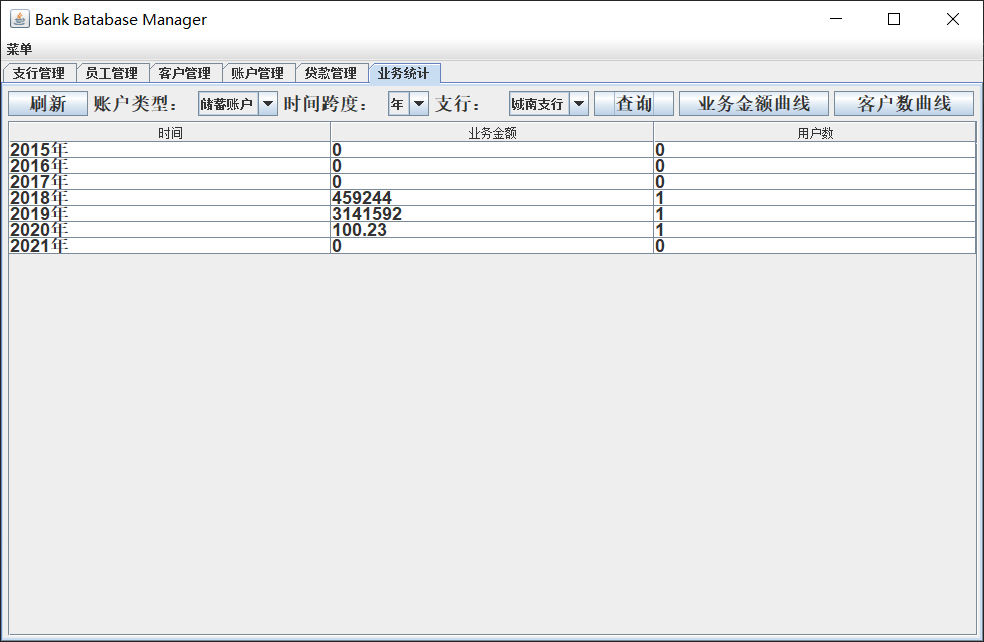
\includegraphics[scale=0.2]{tj1.png}
    \caption{业务统计模块-表格}
\end{figure}
点击“业务金额曲线”,生成对应的业务统计折线图;
\par 
\begin{figure}[H]
    \centering
    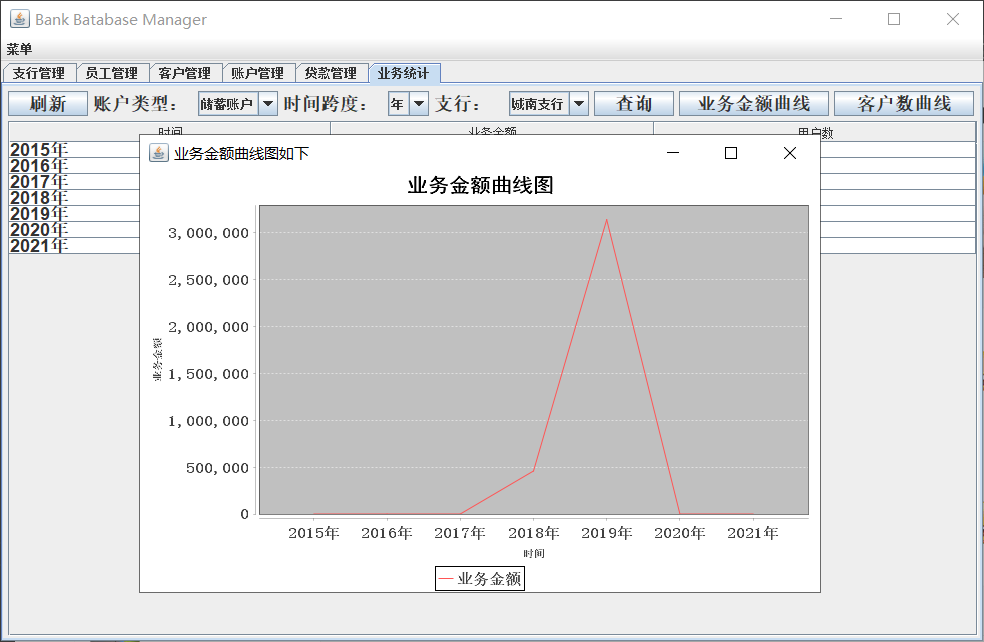
\includegraphics[scale=0.2]{tj2.png}
    \caption{业务统计模块-折线图}
\end{figure}
\subsection{\hei 测试结果}
本部分为部分功能测试。
\subsubsection{\hei 贷款删除测试-发放中}
若贷款业务处于“发放中”,则删除失败。
\begin{figure}[H]
    \centering
    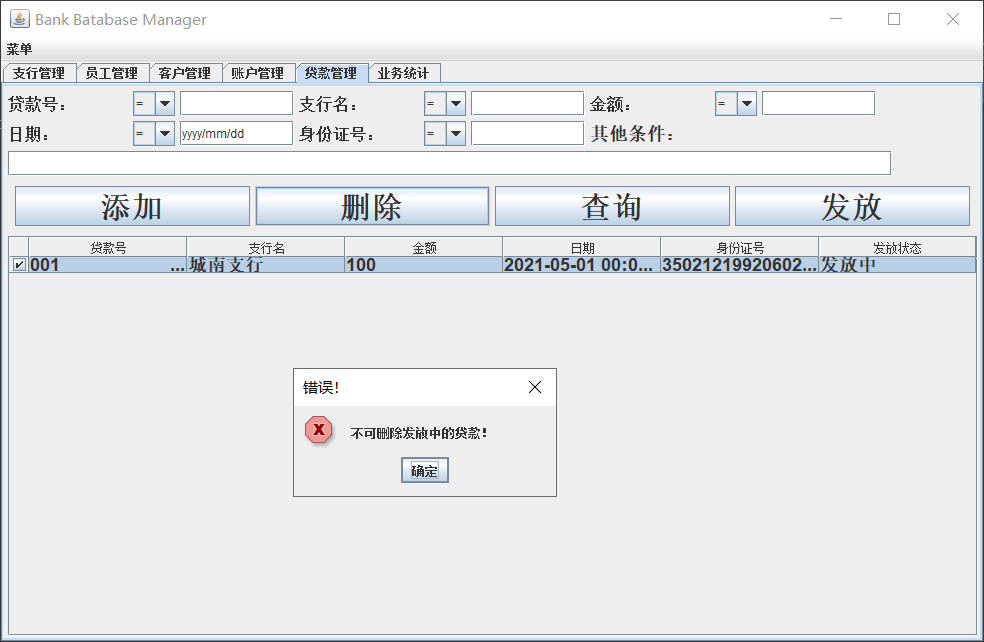
\includegraphics[scale=0.2]{dk333.png}
    \caption{贷款删除测试-发放中}
\end{figure}
\subsubsection{\hei 贷款删除测试-余额不足}
若贷款业务对应的余额不足,小于借款额,则删除失败。
\begin{figure}[H]
    \centering
    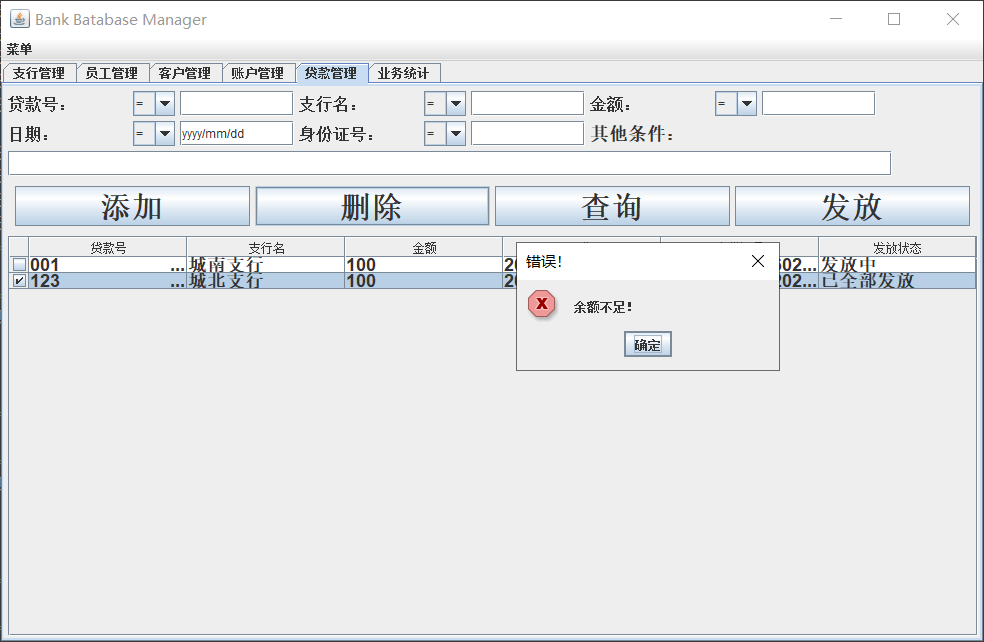
\includegraphics[scale=0.2]{yue.png}
    \caption{贷款删除测试-余额不足}
\end{figure}
\subsubsection{\hei 贷款发放超额测试}
若贷款发放额度超过所给额度,则发放失败。
\begin{figure}[H]
    \centering
    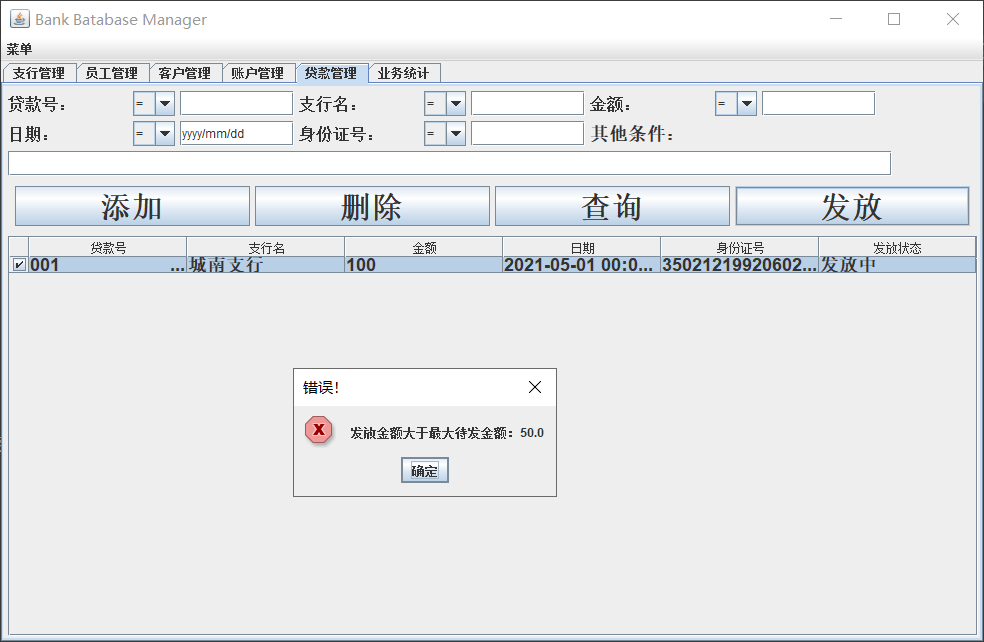
\includegraphics[scale=0.2]{dk4.png}
    \caption{贷款发放超额测试}
\end{figure}
\subsubsection{\hei 添加关联测试}
若添加的实例不满足约束条件,
\begin{figure}[H]
    \centering
    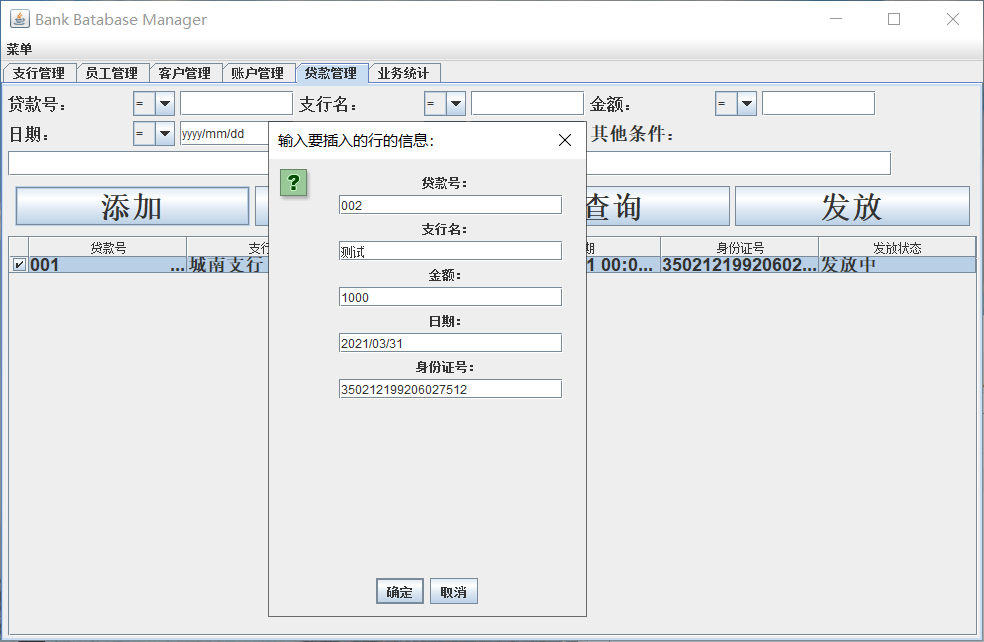
\includegraphics[scale=0.2]{tianj.png}
    \caption{添加关联测试-添加}
\end{figure}
\par 则返回错误信息。
\begin{figure}[H]
    \centering
    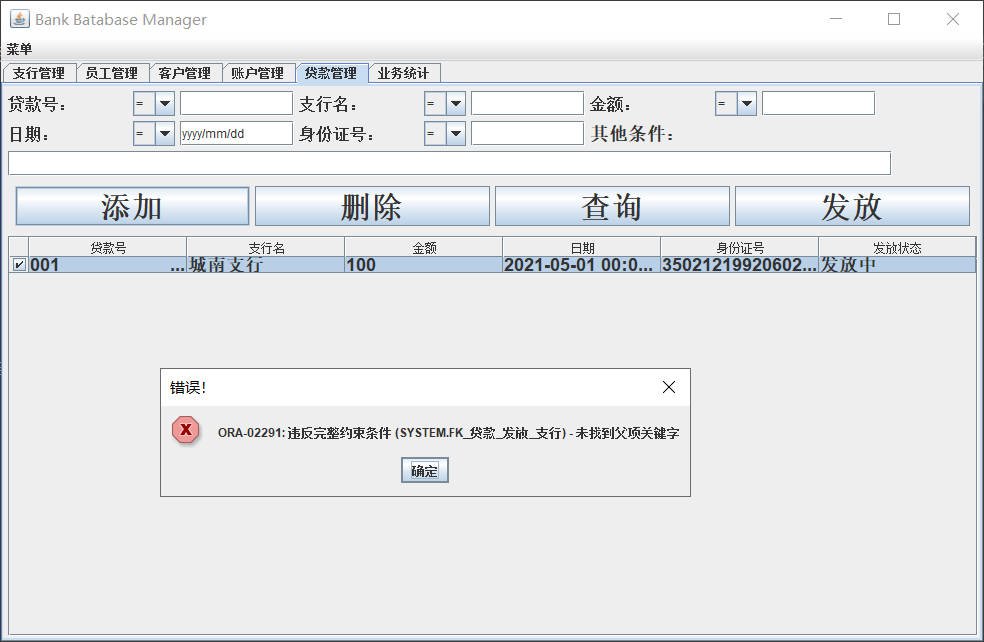
\includegraphics[scale=0.2]{tianj2.png}
    \caption{添加关联测试-错误信息}
\end{figure}
\subsection{\hei 实现中的难点问题及解决}
\subsubsection{\hei 贷款的发放与删除}
在本系统的设计中,对关系模型进行了简化,在处理贷款发放及删除过程中,对应的支票账户余额及透支额的更新便较为复杂。
\par 
又因本次实验采用的是以前段为主的数据库系统模块结构,故在前段实现这些数据的计算。先通过查询支票账户,拥有账户等表,得到所需
数据,计算是否满足贷款发放或删除条件。若满足,则更新对应的支票账户,贷款表,否则返回对应的错误信息。
\section{\hei 总结与讨论}
本次实验在实验二的模式设计基础上继续完成银行业务管理系统的设计,并最终实现了一个C/S架构的系统。在这一过程中,充分理解了数据库设计的优劣,对实验难度的影响,体会到实验二的意义所在。
\par 在实验过程中,也进一步掌握Java,Oracle,PL/SQL等语言和工具的使用,对未来的课程学习和工作受益匪浅。
\end{document}